\documentclass[a4paper,
fontsize=11pt,
%headings=small,
oneside,
numbers=noperiodatend,
parskip=half-,
bibliography=totoc,
final
]{scrartcl}

\usepackage[babel]{csquotes}
\usepackage{synttree}
\usepackage{graphicx}
\setkeys{Gin}{width=.7\textwidth} %default pics size

\graphicspath{{./plots/}}
\usepackage[ngerman]{babel}
\usepackage[T1]{fontenc}
%\usepackage{amsmath}
\usepackage[utf8x]{inputenc}
\usepackage [hyphens]{url}
\usepackage{booktabs} 
\usepackage[left=2.4cm,right=2.4cm,top=2.3cm,bottom=2cm,includeheadfoot]{geometry}
\usepackage{eurosym}
\usepackage{multirow}
\usepackage[ngerman]{varioref}
\setcapindent{1em}
\renewcommand{\labelitemi}{--}
\usepackage{paralist}
\usepackage{pdfpages}
\usepackage{lscape}
\usepackage{float}
\usepackage{acronym}
\usepackage{eurosym}
\usepackage{longtable,lscape}
\usepackage{mathpazo}
\usepackage[normalem]{ulem} %emphasize weiterhin kursiv
\usepackage[flushmargin,ragged]{footmisc} % left align footnote
\usepackage{ccicons} 
\setcapindent{0pt} % no indentation in captions

%%%% fancy LIBREAS URL color 
\usepackage{xcolor}
\definecolor{libreas}{RGB}{112,0,0}

\usepackage{listings}

\urlstyle{same}  % don't use monospace font for urls

\usepackage[fleqn]{amsmath}

%adjust fontsize for part

\usepackage{sectsty}
\partfont{\large}

%Das BibTeX-Zeichen mit \BibTeX setzen:
\def\symbol#1{\char #1\relax}
\def\bsl{{\tt\symbol{'134}}}
\def\BibTeX{{\rm B\kern-.05em{\sc i\kern-.025em b}\kern-.08em
    T\kern-.1667em\lower.7ex\hbox{E}\kern-.125emX}}

\usepackage{fancyhdr}
\fancyhf{}
\pagestyle{fancyplain}
\fancyhead[R]{\thepage}

% make sure bookmarks are created eventough sections are not numbered!
% uncommend if sections are numbered (bookmarks created by default)
\makeatletter
\renewcommand\@seccntformat[1]{}
\makeatother

% typo setup
\clubpenalty = 10000
\widowpenalty = 10000
\displaywidowpenalty = 10000

\usepackage{hyperxmp}
\usepackage[colorlinks, linkcolor=black,citecolor=black, urlcolor=libreas,
breaklinks= true,bookmarks=true,bookmarksopen=true]{hyperref}
\usepackage{breakurl}

%meta
%meta

\fancyhead[L]{Redaktion LIBREAS\\ %author
LIBREAS. Library Ideas, 36 (2019). % journal, issue, volume.
\href{http://nbn-resolving.de/}
{}} % urn 
% recommended use
%\href{http://nbn-resolving.de/}{\color{black}{urn:nbn:de...}}
\fancyhead[R]{\thepage} %page number
\fancyfoot[L] {\ccLogo \ccAttribution\ \href{https://creativecommons.org/licenses/by/4.0/}{\color{black}Creative Commons BY 4.0}}  %licence
\fancyfoot[R] {ISSN: 1860-7950}

\title{\LARGE{Editorial \#36: Nachhaltigkeit von Forschungsinfrastrukturen}}% title
\author{Redaktion LIBREAS} % author

\setcounter{page}{1}

\hypersetup{%
      pdftitle={Editorial \#36: Nachhaltigkeit von Forschungsinfrastrukturen},
      pdfauthor={Redaktion LIBREAS},
      pdfcopyright={CC BY 4.0 International},
      pdfsubject={LIBREAS. Library Ideas, 35 (2019).},
      pdfkeywords={Bibliothek,  Nachhaltigkeit, Forschungsinfrastrastrukturen Editorial},
      pdflicenseurl={https://creativecommons.org/licenses/by/4.0/},
      pdfcontacturl={http://libreas.eu},
      baseurl={http://libreas.eu},
      pdflang={de},
      pdfmetalang={de}
     }



\date{}
\begin{document}

\maketitle
\thispagestyle{fancyplain} 

%abstracts

%body
Vor rund sieben Jahren standen wir vor der Frage, wie wir die LIBREAS
nachhaltig aufstellen können, weil der Serverbetrieb nicht mehr
gewährleistet werden konnte. Wir mussten daher einen Weg finden, die
Zeitschrift zu migrieren und ihre Integrität zu gewährleisten. Klar,
Geld war nicht vorhanden und unsere Zeit sowie unser Know-How waren
begrenzt.

Passend zur Ausgabe \#23 zum Thema Forschungsdatenmanagement\footnote{\url{https://libreas.eu/ausgabe23/}}
überführten wir damals das Journals mittels eines statischen Website
Site-Generator nach GitHub Pages\footnote{\url{https://github.com/libreas/libreas.github.io/}},
welches ein kostenfreies Hosting von statischen Webseiten anbietet.
Pandoc, ein Konvertierungstool für Dokumentenformate\footnote{\url{https://pandoc.org/}},
bildete das Werkzeug, das uns seitdem beim semi-automatischen Setzen der
Artikel hilft\footnote{\url{https://github.com/libreas/libreas.github.io/wiki/Workflow-Satz}}.
Und klar, auch Slack und Google Docs sind für unsere Kommunikationen und
der inhaltlichen Textarbeit unersetzlich. PDFs werden zudem auf dem
edoc-Server der HU Berlin archiviert\footnote{\url{https://edoc.hu-berlin.de/handle/18452/149}}.

Sind Workflow einschließlich der Verbreitung der LIBREAS jetzt also
nachhaltig? Finanziell dank des Vereins, der freiwilligen Arbeit und
fehlenden Kosten fürs Hosting und Setzen bestimmt. Der Umfang der
Redaktion ist stabil und offen für neue Personen. Technisch steht zum
15jährigen Jubiläum eine Aktualisierung an, da seit 2013 vieles passiert
ist. Inhaltlich planen wir bereits die Ausgabe \#38. Für die Ausgabe
\#37 zum Thema \enquote{Forschung und Öffentliche Bibliothek} gibt es
bereits einen Call for Paper\footnote{\url{https://libreas.wordpress.com/2019/11/06/cfp-37-forschung-und-oeffentliche-bibliothek/}}.

\begin{figure}
\centering
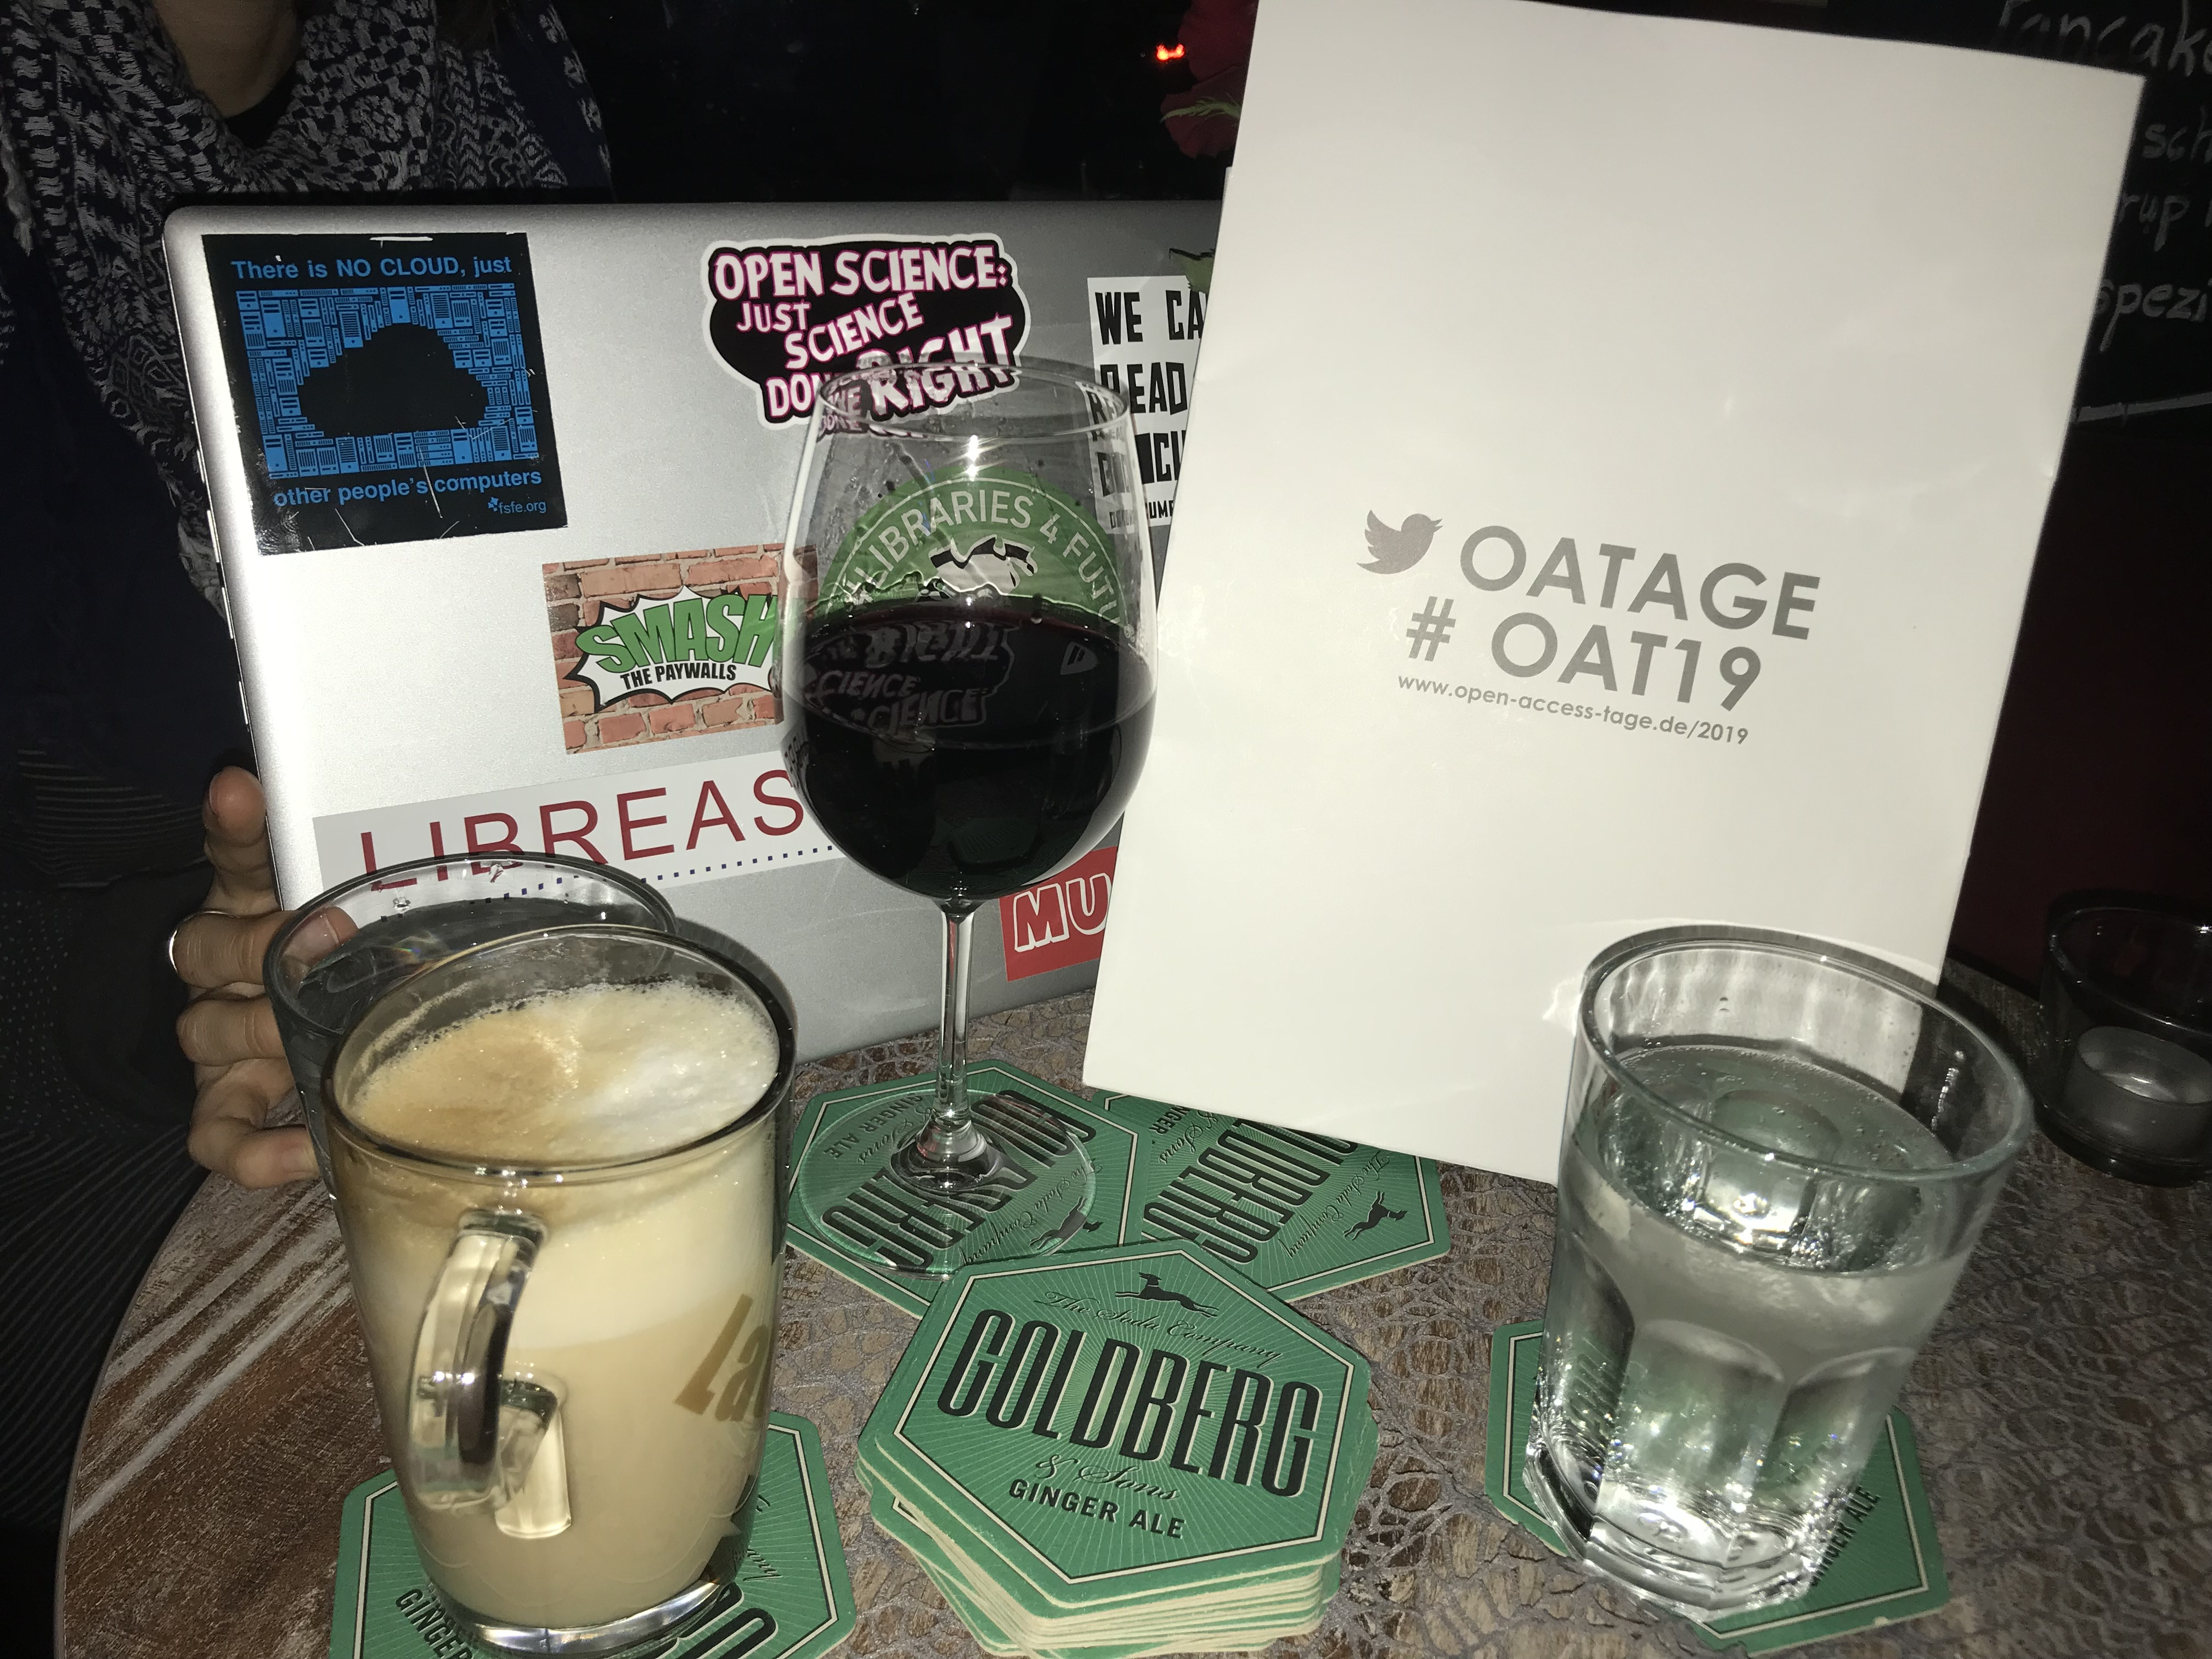
\includegraphics{abb.jpg}
\caption{Redaktionsorte XV. Hannover, Oktober 2019}
\end{figure}

Unter den Beiträgen zum aktuellen Schwerpunkt \enquote{Nachhaltigkeit
von Forschungsinfrastrukturen} finden sich Vorschläge zur
Qualitätssicherung und Finanzierung von Open-Access-Zeit\-schriften
(Kathrin Ganz, Marcel Wrzesinski \& Markus Rauchecker) und
Repositorienplattformen (Beate Rajski \& Pascal Becker). Niklas K.
Hartmann entwickelt Handlungsoptionen zum Umgang mit personenbezogenen
Forschungsdaten. Er verweist auf die Bedeutung von Standards für ein
nachhaltiges Forschungsdatenmanagements, einen Aspekt, den auch
Francesco Gelati und Bernd Kulawik in ihren Beiträgen aufgreifen. Andrea
Bertino und Jan Rohden stellen den DARIAH-DE Helpdesk vor, der die
Nutzung digitaler Werkzeuge und Ressourcen befördern soll. Es gibt zudem
eine Reihe von Interviews und Veranstaltungshinweisen zum Thema
Nachhaltigkeit von Forschungsinfrastrukturen.

Wir finden, dass LIBREAS \#36 damit durchaus eine bemerkenswerte
Sammlung an Beiträgen vereint. Wir wünschen viel Freude und
Denkanregungen!

Ihre / eure Redaktion LIBREAS. Library Ideas

(Aarhus, Berlin, Chur, Dresden, München)

%autor

\end{document}
